% !TEX TS-program = pdfLaTeX+MakeIndex+BibTeX 
\documentclass[11pt,compress,UTF8]{beamer}

\usecolortheme{seahorse}
\useinnertheme[shadow]{rounded}  
\useoutertheme[subsection=false]{smoothbars}
\setbeamertemplate{caption}[numbered] % 序号
\setbeamercovered{transparent=15}
\setbeamersize{text margin left=0.6cm, text margin right=0.6cm} % 设置页边距

\usepackage{ragged2e}
\renewcommand{\raggedright}{\leftskip=0pt \rightskip=0pt plus 0cm} % 对齐
\usepackage{natbib} % 参考文献
\usepackage{gradientframe} % 图片立体感
\graphicspath{{figure/}} % 图片路径

\title{Spatial Generalized Linear Mixed Models with Application to Prevalence Mapping}

\author{Xiang-Yun Huang \and Zai-Xing Li}

\date{
\includegraphics[width=10ex,interpolate=true]{logo} \\ ~~ \\
\today \\ Department of Statistics, School of Science \\ China University of Mining and Technology,Beijing}

\subject{prevalence mapping}
\keywords{Mixed models}

\begin{document}
\raggedright

\maketitle

\begin{frame}
\textbf{Outline}
\begin{enumerate}
  \item Introduction (Motivations and goals)
  \item Literature reviews  
  \item Geostatistical model (SGLMM)
  \item Computing details and simulations
  \item Real data analysis (Applications)
  \item Discussion
\end{enumerate}
\end{frame}


\section{Introduction}

\subsection{Motivations}

\begin{frame}
\textbf{Motivations}

\begin{enumerate}
\item Radionuclide concentrations on Rongelap Island
\item Childhood malaria in the gambia
\item Loa loa prevalence in Cameroon and surrounding areas
\end{enumerate}

\textbf{Goals}
\begin{enumerate}
\item parameter estimation and spatial prediction as \citet{Diggle2016}
\item thesis as \citet{Varin2005}
\end{enumerate}

\end{frame}


\section{Geostatistical model (SGLMM)}

\subsection{Models}
\begin{frame}

{\color{red} \textbf{Multiple prevalence surveys}} \\
Sample $n_{i}$ individuals,observe $Y_{i}$ positives,$i=1,2,\cdots,m$
$$Y_{i}\sim \mathrm{Bin}(n_{i},p_{i})$$

{\color{red} \textbf{Extra-binomial variation}} \\
Sample $n_{i}$ individuals,observe $Y_{i}$ positives,$i=1,2,\cdots,m$
$$Y_{i}|d_{i},U_{i}\sim \mathrm{Bin}(n_{i},p_{i}) \quad 
\log\{p_{i}/(1-p_{i})\}=d_{i}'\beta+U_{i} \quad U_{i} \sim N(0,\tau^2)$$

\textbf{notations:} Spatial Generalized Linear Mixed Models (SGLMM)
\begin{itemize}
\item Latent spatially correlated process \\
Stationary Gaussian Process: $S(x) \sim \mathrm{SGP}\{0,\sigma^2,\rho(u)\} $ \\
correlation function: e.g. $\rho(u)=\exp(-|u|/\phi)$ 
\item Linear prediction (regression model)\\
$d(x)=$ covariates at location $x$\\
Linear prediction: $\eta(x)=d(x)'\beta + S(x)$ \\
Link function: logit $p(x)=\log\{\eta(x)/[1-\eta(x)]\}$ 
\item Conditional distribution for positive proportion $Y_{i}/n_{i}$\\
$Y_{i}|S(\cdot) \sim \mathrm{Bin}(n_{i},p(x_{i}))$ (binomial sampling)
\end{itemize}

\end{frame}


\begin{frame}  % 
\textbf{Standard geostatistical prevalence sampling model:}\\
$$\log[p(x_i)/\{1-p(x_i)\}]=T_{i}=d(x_i)'\beta+S(x_i)+U_{i} $$ \\
$E[Y_{i}|S(x_i),U_{i}]=n_{i}p_{i}$\\
\textbf{theoretical variograms:}
\begin{equation*}
\begin{aligned}
V(x,x')&=\frac{1}{2}\mathrm{Var}\{S(x)-S(x')\}\\
&=\frac{1}{2}\mathrm{Cov}(S(x)-S(x'),S(x)-S(x'))\\
&=\frac{1}{2}\{E[S(x)-S(x')][S(x)-S(x')]-[E(S(x)-S(x'))]^2\}\\
&=\sigma^2-\mathrm{Cov}(S(x),S(x'))=\sigma^2\{1-\rho(u)\},u=||x-x'|| \\
V_{T}(u_{ij})&=\frac{1}{2}\mathrm{Var}\{T_{i}(x)-T_{j}(x)\}
=\frac{1}{2}E[(T_{i}-T_{j})^2]=\tau^2+\sigma^2(1-\rho(u_{ij}))
\end{aligned}
\end{equation*}
\textbf{covariance matrix:}
$$\mathrm{Cov}(T_{i}(x),T_{i}(x)) = \sigma^2+\tau^2, \mathrm{Cov}(T_{i}(x),T_{j}(x))=\sigma^2\rho(u_{ij})$$
% \textbf{empirical variograms:}
% $V_{T}(u)=\frac{1}{2}E[(Y_{i}-Y_{j})^2]$ stationary assumption \\
% $v_{ij}=\frac{1}{2}(Y_{i}-Y_{j})^2$ unbiased estimation 
\end{frame}

\begin{frame}
Mat\'ern class of correlation functions: $$\rho(u)=\{2^{\kappa -1}\Gamma(\kappa)\}^{-1}(u/\phi)^{\kappa}\mathcal{K}_{\kappa}(u/\phi),u > 0$$
\begin{figure}
\centering
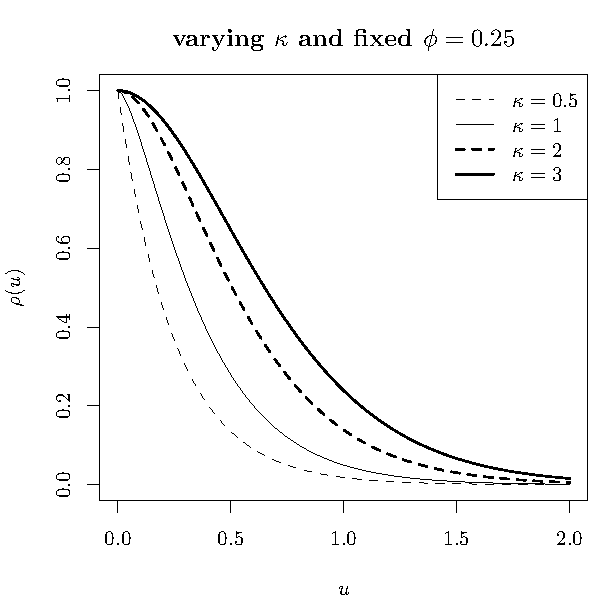
\includegraphics[width=.45\textwidth]{matern1}
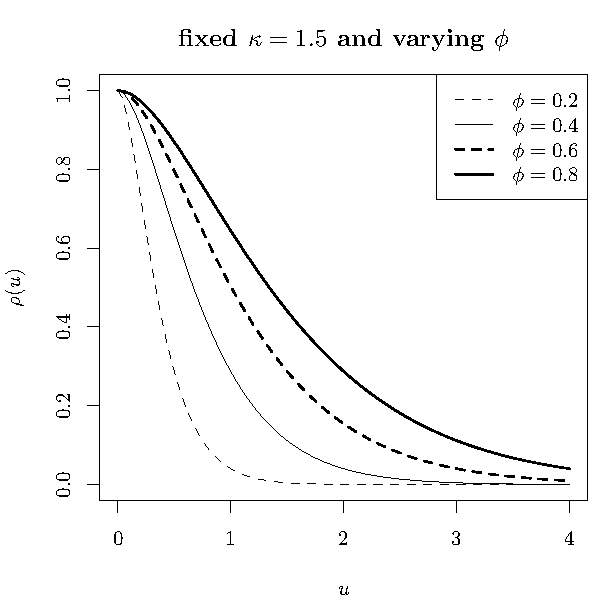
\includegraphics[width=.45\textwidth]{matern2}
\end{figure}
\end{frame}


\begin{frame}
\begin{figure}
\centering
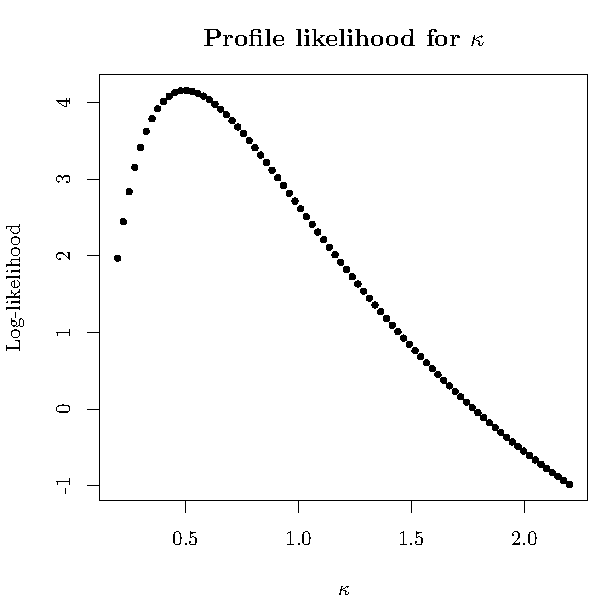
\includegraphics[width=.65\textwidth]{kappa}
\caption{$\kappa=0.4988445$,Loa loa data from \cite{R-PrevMap}}
\end{figure}
\end{frame}


\begin{frame}
\begin{figure}
\centering
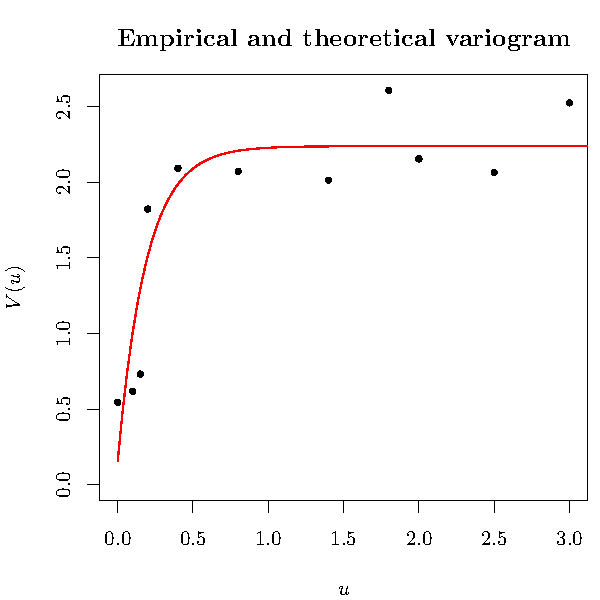
\includegraphics[width=.65\textwidth]{variogram}
\caption{$\tau^2=0.1554,\sigma^2=2.0827,\phi=0.189$ and fixed $\kappa=0.5$}
\end{figure}
\end{frame}
 

\subsection{Computing details and simulations}

\begin{frame}
\textbf{Goals:}
\begin{itemize}
\item estimation: the coefficient vector, 95\% confidence intervals 
\item prediction: probability of Loa loa prevalence of unknown locations 
\end{itemize}

\textbf{Likelihood-based methods inferences} 
\begin{itemize}
\item Monte Carlo EM gradient used by \citet{Zhang2002On}
\item Monte Carlo maximum likelihood used by \citet{Christensen2004} and \citet{Diggle2016}
\item Approximate Monte Carlo EM gradient used by \citet{Hosseini2016}
\end{itemize}

\textbf{Approximate Bayesian Inference}
\begin{itemize}
\item Bayesian approach combined with MCMC methods used by \citet{Diggle1998,Diggle2002}
\item Bayesian approach combined with integrated nested Laplace approximations 
used by \citet{Eidsvik2009Approximate,Rue2009,Rue2017arXiv}
\end{itemize}
\end{frame}


\begin{frame}{Monte Carlo Maximum Likelihood (MCML)}
let $\theta^{\top}=(\sigma^2,\phi,\tau^2)$ , $D$ denote the $n$ by $p$ matrix of covariates, 
$y^{\top}=(y_1,y_2,\cdots,y_n)$ and marginal distribution of $T$ is $N(D\beta,\Sigma(\theta))$.
The conditional distribution of $Y^{\top}=(Y_1,\cdots,Y_n)$ given $T^{\top}=t^{\top}=(t_1,t_2,\cdots,t_n)$ is $$f(y|t)=\prod_{i=1}^{n}f(y_{i}|t_{i})$$  
a product of independent binomial probability functions.\\

The likelihood function for $\beta$ and $\theta$
\begin{equation*}
\begin{aligned}
L(\beta,\theta)& =f(y;\beta,\theta)=\int_{\mathbb{R}^{n}} N(t;D\beta,\Sigma(\theta))f(y|t)dt\\
& = \int_{\mathbb{R}^{n}} \frac{N(t;D\beta,\Sigma(\theta))f(y|t)}{N(t;D\beta_{0},\Sigma(\theta_{0}))f(y|t)}f(y,t)dt\\
& \varpropto \int_{\mathbb{R}^{n}} \frac{N(t;D\beta,\Sigma(\theta))}{N(t;D\beta_{0},\Sigma(\theta_{0}))}f(t|y)dt = E_{T|y}\left[\frac{N(t;D\beta,\Sigma(\theta))}{N(t;D\beta_{0},\Sigma(\theta_{0}))}\right]
\end{aligned}
\end{equation*}
\end{frame}

\begin{frame}{Computing details}

fixed $\beta_{0},\theta_{0}$,then we get the joint distribution of $Y$ and $T$ 
$$f(y,t)=N(t;D\beta_{0},\Sigma(\theta_{0}))f(y|t)$$ for pre-defined and use MCMC algorithm
to obtain $m$ samples $t_{i}$ from conditional distribution of $T$ given $Y=y$ under $\beta_{0}$ and 
$\theta_{0}$, so $$L_{m}(\beta,\theta)=\frac{1}{m}\sum_{i=1}^{n}\frac{N(t_{i};D\beta,\Sigma(\theta))}{N(t_{i};D\beta_{0},\Sigma(\theta_{0}))}$$

Let $\hat{\beta}_{m}$ and $\hat{\theta}_{m}$ denote MCML estimates by maximising $L_{m}(\beta,\theta)$
given an suitable initial values $\beta_{0}$ and $\theta_{0}$, repeat the iterative procedure with 
$\beta_{0}=\hat{\beta}_{m}$ and $\theta_{0}=\hat{\theta}_{m}$ until convergence.\\

For maximization of $L_{m}(\beta,\theta)$, we can choose BFGS algorithm or unconstrained optimization with PORT rountines.
\end{frame}


\section{Real data analysis (Applications)}

\subsection{Loa loa prevalence data}

\begin{frame}{Case Study 1}{Loa loa prevalence data from 197 village surveys in west Africa, \citet{Diggle2007a}}
\begin{table}
\footnotesize
\vspace{-1em}
\caption{\label{tab:Loaloa}Loa loa prevalence data (partial)}
\vspace{-1.5em}
\centering
\begin{tabular}[t]{c|c|c|c|c|c}
\hline
LONGITUDE & LATITUDE & NO\_EXAM & NO\_INF & ELEVATION & MAX9901\\
\hline
8.0419 & 5.7367 & 162 & 0 & 108 & 0.69\\
\hline
8.0043 & 5.6803 & 167 & 1 & 99 & 0.74\\
\hline
8.9056 & 5.3472 & 88 & 5 & 783 & 0.79\\
\hline
8.1007 & 5.9174 & 62 & 5 & 104 & 0.67\\
\hline
8.1825 & 5.1045 & 167 & 3 & 109 & 0.85\\
\hline
8.9292 & 5.3556 & 66 & 3 & 909 & 0.80\\
\hline
11.3600 & 4.8850 & 163 & 11 & 503 & 0.78\\
\hline
8.0675 & 5.8978 & 83 & 0 & 103 & 0.69\\
\hline
\end{tabular}
\end{table}

\begin{itemize}
\item MAX9901: Maximum of all NDVI values recorded at village location, 1999-2001.
\item MEAN9901, MIN9901 and STDEV9901 are as defined above.
\item NDVI: normalised-difference vegetation index  
\end{itemize}

\end{frame}

\begin{frame}
\begin{figure}
\centering
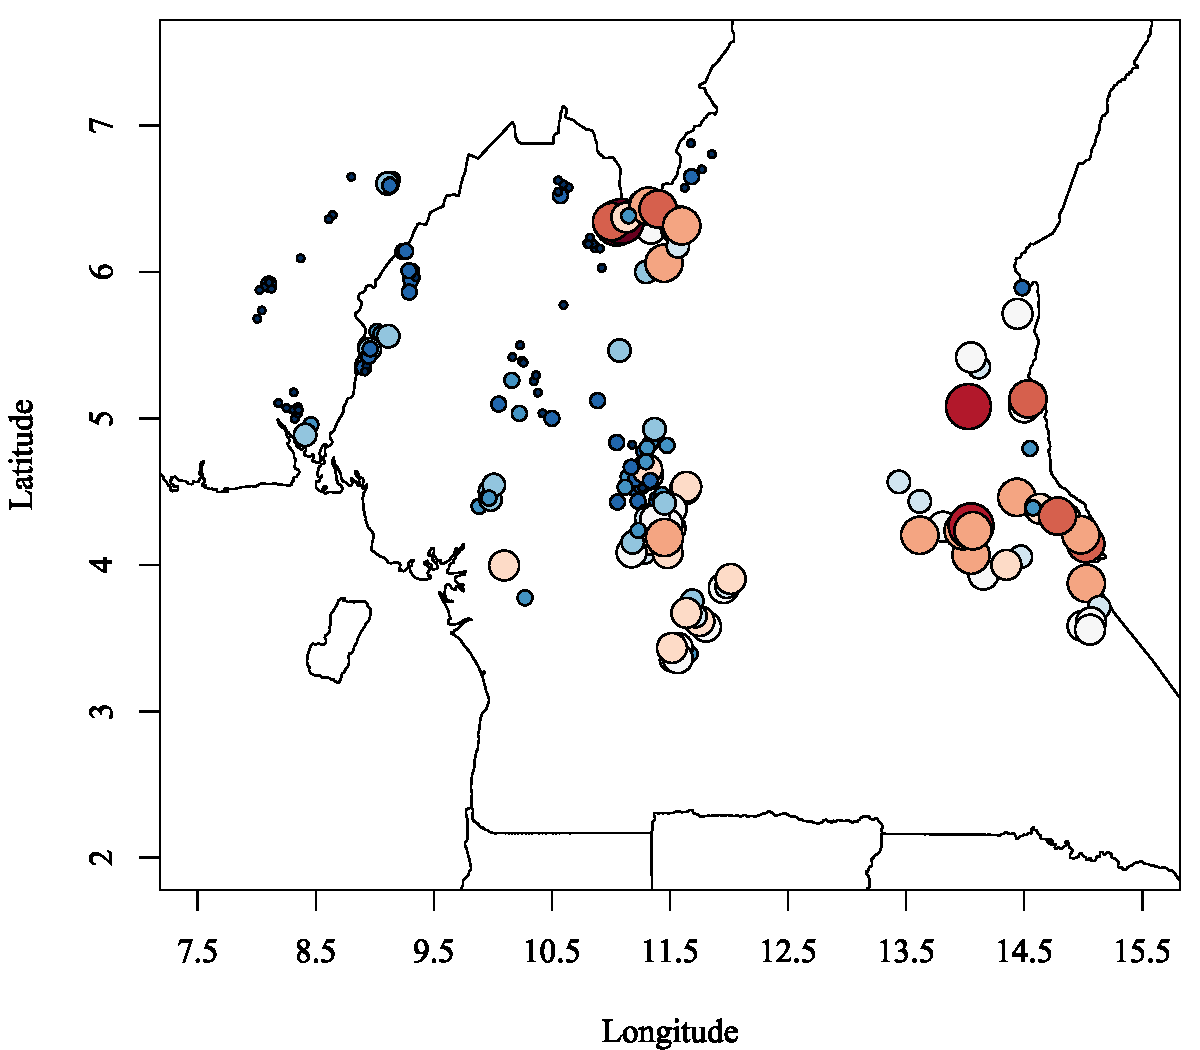
\includegraphics[width=.7\textwidth]{Prevalence00.pdf}
\caption{\footnotesize{cex (size of circles): 0.5, 1.0, 1.5, 2.0, 2.5, 3.0 corresponds to the observed prevalence of Loa loa: [0,0.05), [0.05,0.15), [0.15,0.25), [0.25,0.35), [0.35,0.45), [0.45,0.55) and
policy intervention threshold is 0.2}}
\end{figure}
\end{frame}

\begin{frame}{Statistical Model}
\citet{Diggle2007a}\\
\textbf{Goals:}\\
using spatial statistical methods to address the issue of spatial correlation, 
and using Bayesian methods to quantify the uncertainty 
in the predictions from \citet{Diggle1998} to create a new map.\\
{\color{red} village level model:}
\begin{equation*}
\begin{aligned}
\log\{p(x)/[1-p(x)] \}=& 
\alpha + f_{1}(\mathrm{ELEVATION}) + f_{2}[\max(\mathrm{NDVI})]\\
& + f_{3}[\mathrm{s.d.}(\mathrm{NDVI})]+S(x) % f_{1} f_{2} f_{3} 分段线性 还可以样条 局部多项式平滑
\end{aligned}
\end{equation*}
\begin{itemize}
\item $S(x)$ Gaussian process with mean zero ,variance $\sigma^2$ 
and correlation function  $\mathrm{Corr}(S(x),S(x'))=\exp(-||x-x'||/\phi)+\tau^2/\sigma^2 \cdot \mathrm{I}_{\{x=x'\}}$
\item $f_{1}(\cdot),f_{2}(\cdot)$ and $f_{3}(\cdot)$ are piece-wise linear functions
\end{itemize}

\end{frame}

\begin{frame}
\begin{figure}
\centering
% \gradientframe[padding =2mm]{\includegraphics<1-1>[width=.7\textwidth]{Prevalence01}}
% \gradientframe[padding =2mm]{\includegraphics<2-2>[width=.7\textwidth]{Prevalence02}}
\gradientframe[padding =2mm]{\includegraphics<1-1>[width=.7\textwidth]{Prevalence0202}}
\gradientframe[padding =2mm]{\includegraphics<2-2>[width=.7\textwidth]{Prevalence03}}
\gradientframe[padding =2mm]{\includegraphics<3-3>[width=.7\textwidth]{Prevalence04}}
% \gradientframe[padding =2mm]{\includegraphics<4-4>[width=.7\textwidth]{Prevalence05}}
\end{figure}
\end{frame}

\begin{frame}
\begin{figure}
\centering
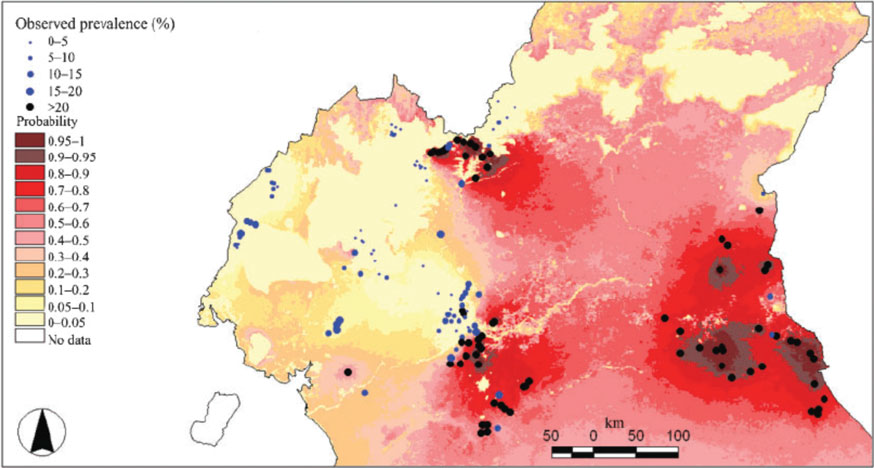
\includegraphics[width=.9\textwidth]{Loaloa}
\caption{Predictive probability map of Loa loa prevalence in Cameroon and surrounding areas (adapted from \citet{Diggle2007a} ). Empirical prevalences at surveyed locations are indicated by size and color coded dots.}
\end{figure}
\end{frame}



\subsection{Childhood malaria in the gambia}
\begin{frame}{Case Study 2}{Childhood malaria in the gambia, \citet{Diggle2002}}
\begin{table}
\footnotesize
\vspace{-1em}
\caption{\label{tab:gambia}Childhood malaria data (partial)}
\vspace{-1em}
\centering
\begin{tabular}[t]{l|c|c|c|c|c|c|c|c}
\hline
  & x & y & pos & age & netuse & treated & green & phc\\
\hline
1850 & 349631.3 & 1458055 & 1 & 1783 & 0 & 0 & 40.85 & 1\\
\hline
1851 & 349631.3 & 1458055 & 0 & 404 & 1 & 0 & 40.85 & 1\\
\hline
1852 & 349631.3 & 1458055 & 0 & 452 & 1 & 0 & 40.85 & 1\\
\hline
1853 & 349631.3 & 1458055 & 1 & 566 & 1 & 0 & 40.85 & 1\\
\hline
\end{tabular}
\end{table}
\begin{itemize}
\item pos: presence (1) or absence (0) of malaria in a blood sample taken from the child
\item netuse: whether (1) or not (0) the child regularly sleeps under a bed-net.
\item treated: whether (1) or not (0) the bed-net is treated (coded 0 if netuse=0).
\item green: satellite-derived measure of the green-ness of vegetation in the immediate vicinity of the village (arbitrary units).
\item phc: presence (1) or absence (0) of a health center in the village.
\end{itemize}
\end{frame}

\begin{frame}
\frametitle{Statistical Model}
\citet{Diggle2002}
\begin{itemize}
\item the effects of child level covariates (age and bed net use)
\item village level covariates (the primary health care and greenness of surrounding vegetation)
\item separate components for residual spatial
\item non-spatial extrabinomial variation
\end{itemize}
{\color{red}Child level model:}
$$ \log [p_{ij}/(1-p_{ij})] =\alpha + \beta'z_{ij} + U_{i} + S(x_{i})$$

\end{frame}



\begin{frame}
\begin{figure}
\centering
\gradientframe[padding =2mm]{\includegraphics<1-1>[width=.7\textwidth]{gambia00}}
\gradientframe[padding =2mm]{\includegraphics<2-2>[width=.7\textwidth]{bed_net}}
\gradientframe[padding =2mm]{\includegraphics<3-3>[width=.7\textwidth]{netuse_treated}}
\gradientframe[padding =2mm]{\includegraphics<4-4>[width=.7\textwidth]{gambia_prevalence}}
\end{figure}
\end{frame}



\section{Discussion}

\subsection{Suggestions}

\begin{frame}
\begin{description}
\item[\textbf{R:}] geoR geoRglm spatial PrevMap \\
\citet{R-geoR,R-geoRglm,R-spatial,Giorgi2016}

\item[\textbf{Stan:}] Stan \footnote{\scriptsize \url{http://mc-stan.org/} }  
interfaces with R (RStan) ,Python (PyStan) , MATLAB (MatlabStan) 
and  more \\ \citet{Stan2015,Stan2017}

\item[\textbf{PyMC3:}] Probabilistic programming in Python using PyMC3 \\ \citet{Salvatier2016}

\item[\textbf{JAGS:}] \textbf{J}ust \textbf{A}nother \textbf{G}ibbs \textbf{S}ampler \footnote{\scriptsize \url{https://en.wikipedia.org/wiki/Just_another_Gibbs_sampler}} \\
Bayesian hierarchical models using Markov chain Monte Carlo (MCMC)
\item[\textbf{BUGS:}] \textbf{B}ayesian inference \textbf{U}sing \textbf{G}ibbs \textbf{S}ampling ,
such as winBUGS, OpenBUGS 
\item[\textbf{R-INLA:}] \textbf{I}ntegrated \textbf{N}ested \textbf{L}aplace \textbf{A}pproximations \\
\citet{Rue2009,R-INLA,Rue2017arXiv}
\end{description}

\end{frame}


\begin{frame}

  \centerline{\Huge\color{red} Thanks }

\end{frame}

\begin{frame}[allowframebreaks]
% pkgs <- c("nlme","lme4","geoR","geoRglm","PrevMap","INLA","spatial")
% write_bib(pkgs, file = "R-GLMM-pkgs.bib")
\bibliographystyle{apalike}
\bibliography{R-GLMM-pkgs}
\end{frame}

\end{document} 